\chapter{Stéréochimie~: chiralité et isomères}\label{ch:g12:stereochemistry}

Les feuilles de menthe verte et les graines de carvi n'ont pas du tout
la même odeur~: l'une est l'odeur fraîche du chewing-gum, l'autre l'odeur
chaude du pain de seigle. Pourtant, la \omterm{def:g7:atoms-and-molecules:molecule}{molécule} responsable de chacune
de ces odeurs est la même carvone, faite des mêmes \omterm{def:g7:atoms-and-molecules:atom}{atomes} liés dans le
même ordre. Les deux carvones ne diffèrent que comme une main gauche
diffère d'une main droite~: chacune est l'image de l'autre dans un
miroir. Notre nez, fait de \omterm{def:g7:atoms-and-molecules:molecule}{molécules} qui ont elles-mêmes une
«~main~», les distingue. Ce chapitre apprend à voir les \omterm{def:g7:atoms-and-molecules:molecule}{molécules} en
trois dimensions.

\begin{recall}
La géométrie des \omterm{def:g7:atoms-and-molecules:molecule}{molécules}, et les triangles pleins et hachurés qui
les dessinent dans l'espace (\cref{ch:g10:lewis-and-shape}). Les
\omterm{def:g11:organic-skeletons:isomer}{isomères de constitution} (\cref{ch:g11:organic-skeletons}). Les \omterm{def:g11:functional-groups:functional-group}{groupes
caractéristiques} (\cref{ch:g11:functional-groups}).
\end{recall}

\begin{omfigure}
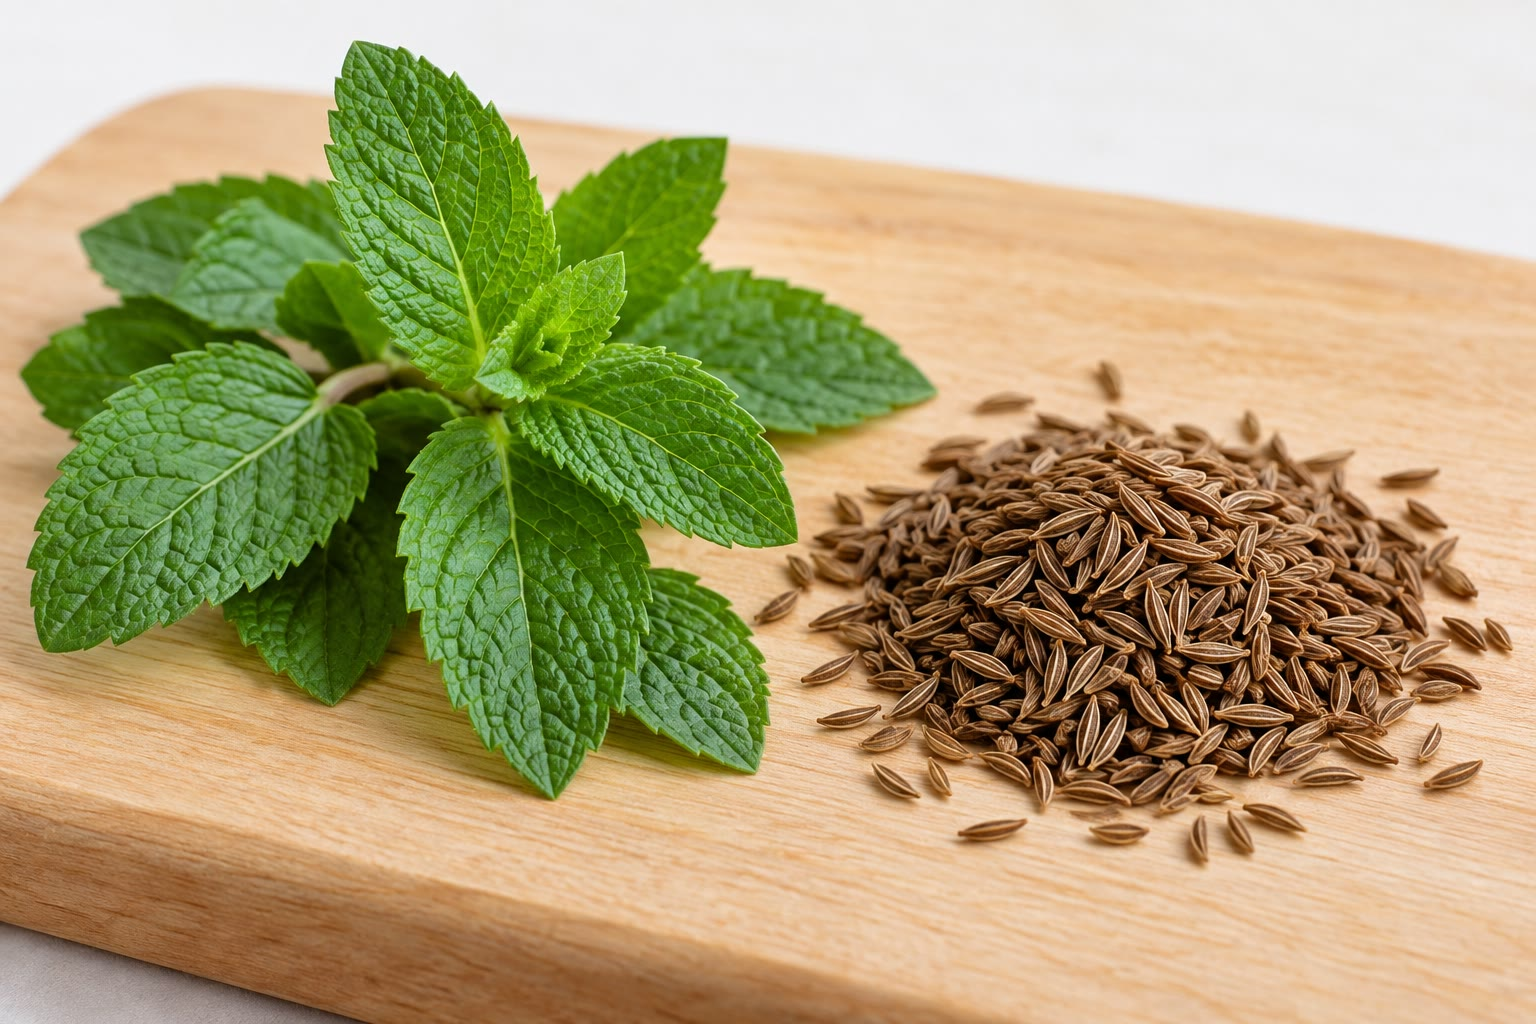
\includegraphics[width=0.48\linewidth]{images/book1/ai/g12-mint-caraway.jpg}

{\small Menthe verte et carvi~: deux \omterm{def:g7:atoms-and-molecules:molecule}{molécules} images l'une de l'autre
dans un miroir, deux odeurs.}
\end{omfigure}

\section{Les molécules dans l'espace}

\begin{definition}[Stéréoisomères]\label{def:g12:stereochemistry:stereoisomer}
Des \emph{stéréoisomères}\index{stereoisomere@stéréoisomère} sont des \omterm{def:g7:atoms-and-molecules:molecule}{molécules} qui ont
la même formule et le même enchaînement d'\omterm{def:g7:atoms-and-molecules:atom}{atomes} liés, et qui ne
diffèrent que par la disposition de leurs \omterm{def:g7:atoms-and-molecules:atom}{atomes} dans l'espace.
\end{definition}

\begin{definition}[Représentation de Cram]\label{def:g12:stereochemistry:cram}
Dans la \emph{représentation de Cram}\index{representation de cram@représentation de Cram}
d'un \omterm{def:g7:atoms-and-molecules:atom}{atome} de carbone engagé dans quatre liaisons simples, deux liaisons
sont dessinées dans le plan de la feuille par des traits simples,
formant un angle~; la liaison dirigée vers le lecteur est dessinée par
un triangle plein, et la liaison dirigée vers l'arrière par un triangle
hachuré.
\end{definition}

\section{La chiralité}

\begin{definition}[Chiral, carbone asymétrique]\label{def:g12:stereochemistry:chiral}
Un objet ou une \omterm{def:g7:atoms-and-molecules:molecule}{molécule} est \emph{chiral}\index{chiral} s'il n'est pas
superposable à son image dans un miroir, comme une main. Un \omterm{def:g7:atoms-and-molecules:atom}{atome} de
carbone lié à quatre \omterm{def:g7:atoms-and-molecules:atom}{atomes} ou groupes d'\omterm{def:g7:atoms-and-molecules:atom}{atomes} différents est un
\emph{carbone asymétrique}\index{carbone asymetrique@carbone asymétrique}~; on le repère
souvent par un astérisque.
\end{definition}

\begin{proposition}[Un carbone asymétrique rend une molécule chirale]\label{prop:g12:stereochemistry:one-carbon}
Une \omterm{def:g7:atoms-and-molecules:molecule}{molécule} qui possède exactement un \omterm{def:g12:stereochemistry:chiral}{carbone asymétrique} est chirale.
\end{proposition}

\begin{proof}
Admis~: échanger deux des quatre groupes différents autour du \omterm{def:g12:stereochemistry:chiral}{carbone
asymétrique} donne l'image dans un miroir, et aucune rotation de la
\omterm{def:g7:atoms-and-molecules:molecule}{molécule} entière ne permet de revenir à la \omterm{def:g7:atoms-and-molecules:molecule}{molécule} de départ, puisque
les quatre groupes sont tous différents.
\end{proof}

\begin{definition}[Énantiomères, mélange racémique]\label{def:g12:stereochemistry:enantiomer}
Deux \omterm{def:g12:stereochemistry:stereoisomer}{stéréoisomères} images l'un de l'autre dans un miroir et non
superposables sont des \emph{énantiomères}\index{enantiomere@énantiomère}. Un
\omterm{def:g6:pure-substances-and-mixtures:mixture}{mélange} de quantités égales de deux énantiomères est un \emph{mélange
racémique}\index{melange racemique@mélange racémique}.
\end{definition}

\begin{omfigure}
\setchemfig{atom sep=2.2em}
\begin{tikzpicture}[font=\small]
  \node at (-2.4,0) {\chemfig{C(-[2]COOH)(-[4]H_3C)(<[:-30]OH)(<:[:-150]H)}};
  \node at (2.4,0) {\chemfig{C(-[2]COOH)(-[0]CH_3)(<[:-150]HO)(<:[:-30]H)}};
  \draw[dashed, omDef, thick] (0,-1.5) -- (0,1.6) node[above] {miroir};
  \node[anchor=north] at (-2.4,-1.4) {acide lactique, A};
  \node[anchor=north] at (2.4,-1.4) {son image dans un miroir, B};
\end{tikzpicture}

{\small Les deux \omterm{def:g12:stereochemistry:enantiomer}{énantiomères} de l'acide lactique,
\ce{CH3-CH(OH)-COOH}, en \omterm{def:g12:stereochemistry:cram}{représentation de Cram}. Le carbone central est
asymétrique (\ce{H}, \ce{OH},
\ce{CH3}, \ce{COOH}). Aucune rotation ne transforme A en B~: ils sont
aussi différents qu'une main gauche et une main droite.}
\end{omfigure}

\begin{method}[Une molécule est-elle chirale~?]\label{met:g12:stereochemistry:chiral}
\begin{enumerate}
  \item Chercher les \omterm{def:g12:stereochemistry:chiral}{carbones asymétriques}~: un carbone portant quatre
        groupes différents. Aucun~: la \omterm{def:g7:atoms-and-molecules:molecule}{molécule} n'est pas chirale (dans
        ce livre).
  \item Exactement un~: la \omterm{def:g7:atoms-and-molecules:molecule}{molécule} est chirale.
  \item Deux ou plus~: chercher un plan qui coupe la \omterm{def:g7:atoms-and-molecules:molecule}{molécule} en deux
        moitiés images l'une de l'autre, dans l'une de ses \omterm{def:g12:stereochemistry:conformation}{conformations}~;
        s'il en existe un, la \omterm{def:g7:atoms-and-molecules:molecule}{molécule} n'est pas chirale, sinon elle
        l'est.
\end{enumerate}
\end{method}

\begin{remark}[Mêmes propriétés, odeurs différentes]\label{rem:g12:stereochemistry:same}
% ledger: smell:carvone-R, smell:carvone-S
Deux \omterm{def:g12:stereochemistry:enantiomer}{énantiomères} ont les mêmes températures de fusion et d'ébullition,
la même \omterm{def:g6:solutions-and-solubility:solubility}{solubilité}, les mêmes spectres~: toute mesure faite avec un
instrument qui n'est pas lui-même \omterm{def:g12:stereochemistry:chiral}{chiral} donne le même résultat pour les
deux. Ils ne diffèrent que lorsqu'ils rencontrent quelque chose de
\omterm{def:g12:stereochemistry:chiral}{chiral}, comme la lumière polarisée, qu'ils font tourner en sens opposés,
ou les récepteurs du nez~: une carvone sent la menthe verte, son
\omterm{def:g12:stereochemistry:enantiomer}{énantiomère} le carvi.
\end{remark}

\section{Les diastéréoisomères}

\begin{definition}[Diastéréoisomères]\label{def:g12:stereochemistry:diastereomer}
Des \omterm{def:g12:stereochemistry:stereoisomer}{stéréoisomères} qui ne sont pas images l'un de l'autre dans un miroir
sont des \emph{diastéréoisomères}\index{diastereoisomere@diastéréoisomère}.
Contrairement aux \omterm{def:g12:stereochemistry:enantiomer}{énantiomères}, les diastéréoisomères ont des propriétés
physiques différentes.
\end{definition}

\begin{proposition}[Dénombrer les stéréoisomères]\label{prop:g12:stereochemistry:count}
Une \omterm{def:g7:atoms-and-molecules:molecule}{molécule} qui possède $n$ \omterm{def:g12:stereochemistry:chiral}{carbones asymétriques} a au plus $2^n$
\omterm{def:g12:stereochemistry:stereoisomer}{stéréoisomères}. Il y en a moins quand la \omterm{def:g7:atoms-and-molecules:molecule}{molécule} a deux moitiés
identiques~: l'une des combinaisons possède alors un plan de symétrie et
n'est pas chirale (c'est une forme \emph{méso}).
\end{proposition}

\begin{proof}
Chaque \omterm{def:g12:stereochemistry:chiral}{carbone asymétrique} peut prendre deux dispositions,
indépendamment des autres~: $2 \times 2 \times \dots \times 2 = 2^n$ combinaisons. Quand deux
combinaisons sont la même \omterm{def:g7:atoms-and-molecules:molecule}{molécule}, le nombre diminue.
\end{proof}

\begin{omfigure}
\setchemfig{atom sep=1.9em}
\begin{tabular}{ccc}
\chemfig{HOOC-[:-30]C(<[:-90]OH)-[:30]C(<[:90]OH)-[:-30]COOH} &
\chemfig{HOOC-[:-30]C(<:[:-90]OH)-[:30]C(<:[:90]OH)-[:-30]COOH} &
\chemfig{HOOC-[:-30]C(<[:-90]OH)-[:30]C(<:[:90]OH)-[:-30]COOH} \\[4pt]
\small acide L-tartrique & \small acide D-tartrique & \small acide méso-tartrique \\
\small (\omterm{def:g12:stereochemistry:chiral}{chiral}) & \small (\omterm{def:g12:stereochemistry:chiral}{chiral}, image miroir de L) & \small (non \omterm{def:g12:stereochemistry:chiral}{chiral})
\end{tabular}

{\small Les trois \omterm{def:g12:stereochemistry:stereoisomer}{stéréoisomères} de l'acide tartrique. L et D sont
\omterm{def:g12:stereochemistry:enantiomer}{énantiomères}~; chacun est un \omterm{def:g12:stereochemistry:diastereomer}{diastéréoisomère} de la forme méso, qui
possède un plan de symétrie dans l'une de ses \omterm{def:g12:stereochemistry:conformation}{conformations}~: trois
\omterm{def:g12:stereochemistry:stereoisomer}{stéréoisomères}, et non $2^2 = 4$.}
\end{omfigure}

\begin{history}[Pasteur trie des cristaux à la main, 1848]
En 1848, le jeune chimiste Louis Pasteur examina à la loupe des
cristaux d'un sel de l'«~acide racémique~», une forme d'acide tartrique
qui ne faisait tourner la lumière polarisée ni dans un sens ni dans
l'autre. Il remarqua que les cristaux avaient deux formes, images l'une
de l'autre dans un miroir, et les tria un à un avec une pince. Une fois
dissous, l'un des tas faisait tourner la lumière polarisée vers la
droite, l'autre, d'autant, vers la gauche~: l'acide racémique était un
\omterm{def:g6:pure-substances-and-mixtures:mixture}{mélange} de deux \omterm{def:g7:atoms-and-molecules:molecule}{molécules} images l'une de l'autre. Les \omterm{def:g7:atoms-and-molecules:molecule}{molécules},
conclut-il, peuvent avoir une «~main~».
\end{history}

\begin{omfigure}
\begin{minipage}[t]{0.36\linewidth}\centering
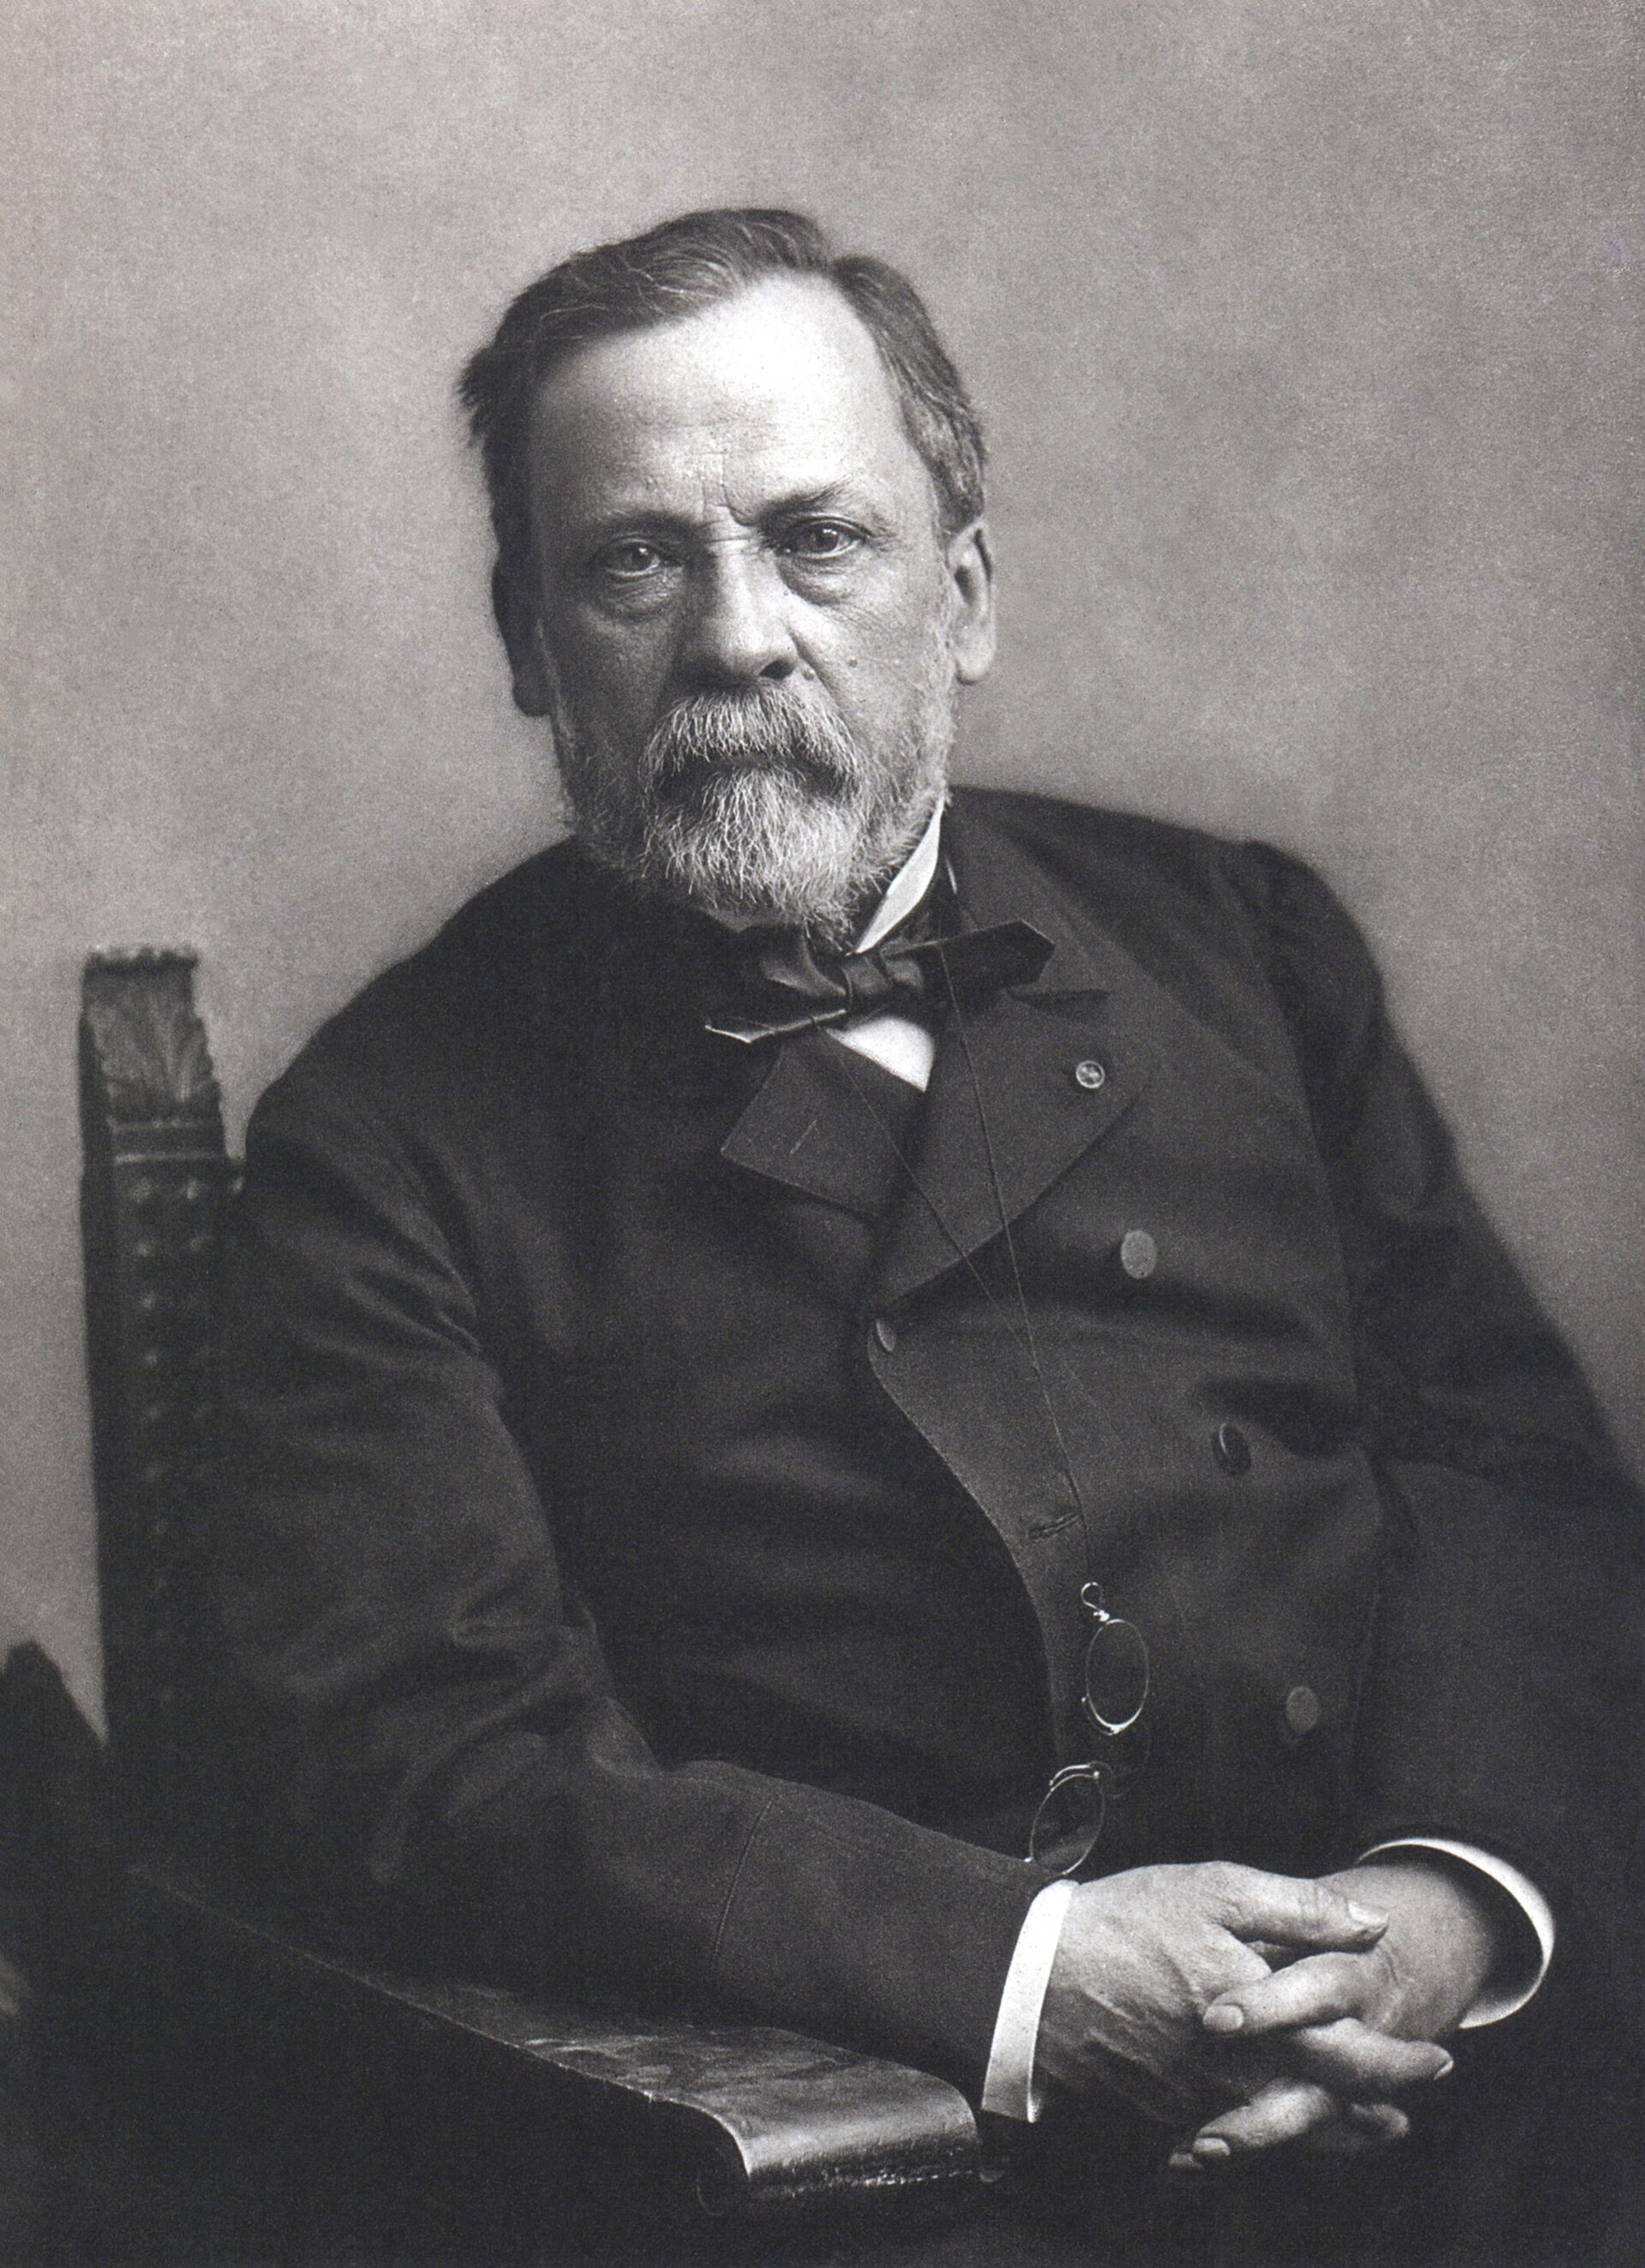
\includegraphics[height=5cm]{images/book1/pasteur.jpg}

{\small Louis Pasteur (1822--1895), photographié par Paul Nadar.}
\end{minipage}\qquad
\begin{minipage}[t]{0.36\linewidth}\centering
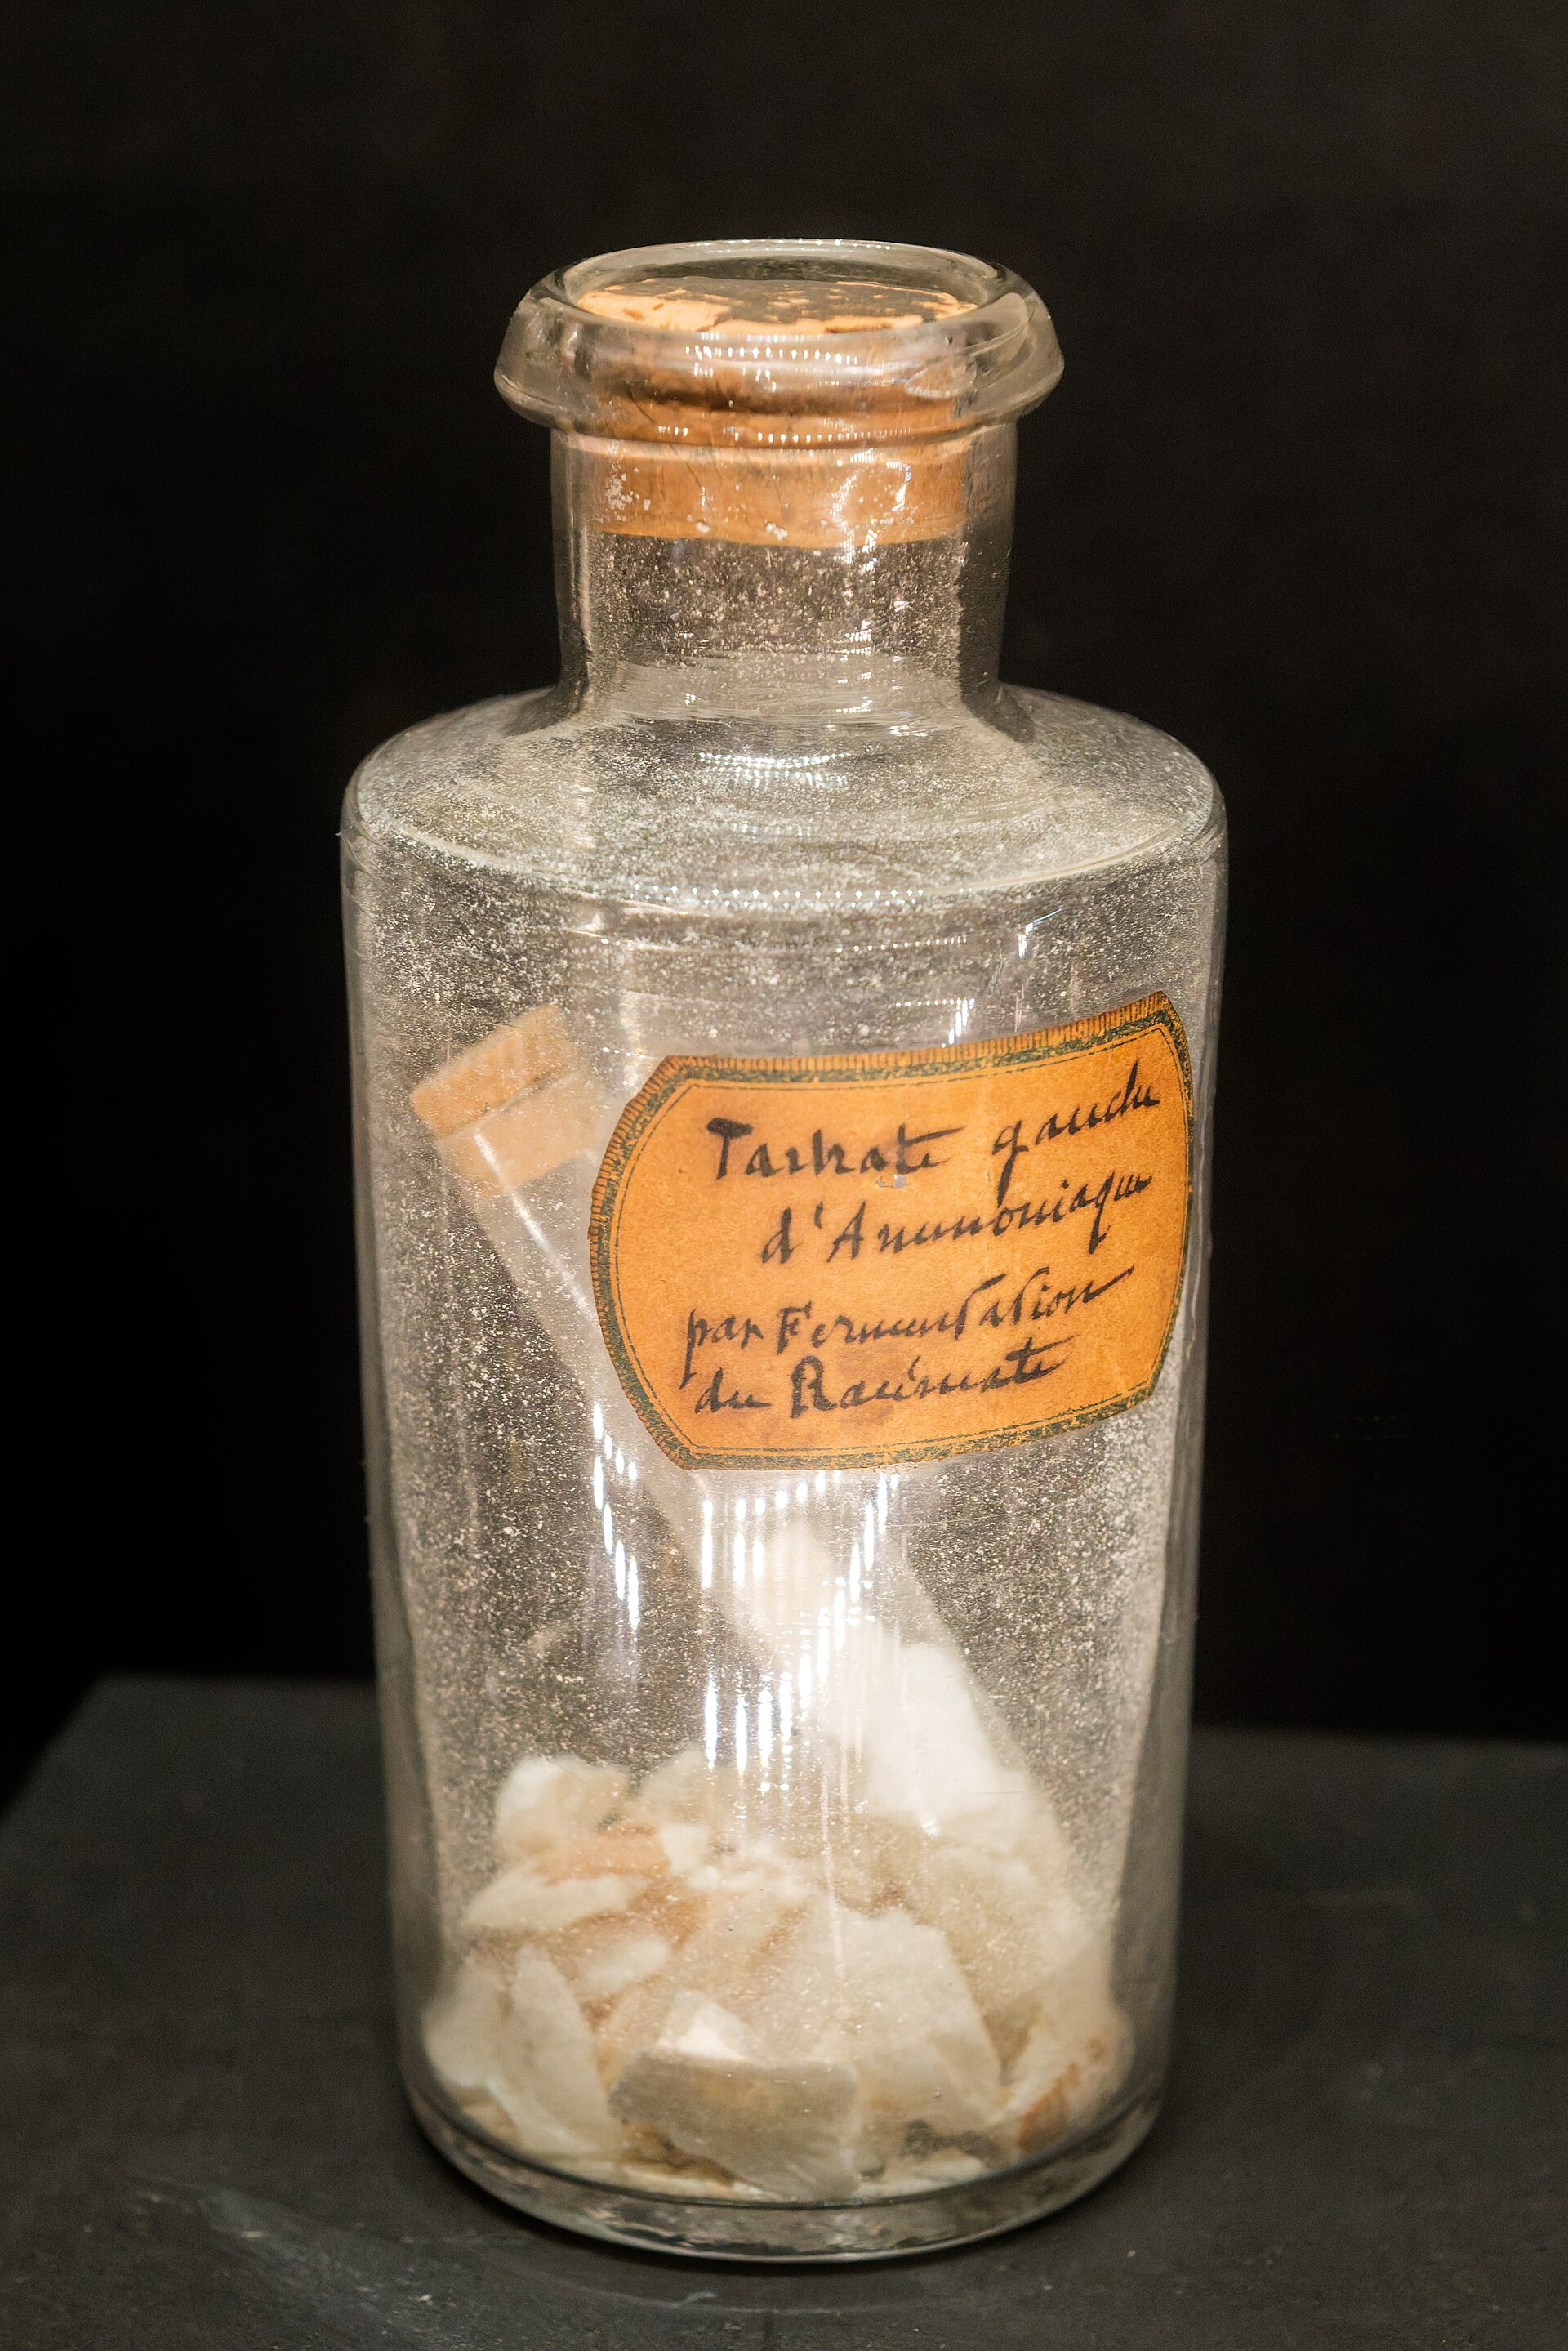
\includegraphics[height=5cm]{images/book1/tartrate-crystals.jpg}

{\small Cristaux de tartrate d'ammonium de la collection de Pasteur.
Photo Marie-Lan Taÿ Pamart, CC BY 4.0.}
\end{minipage}
\end{omfigure}

\section{Les isomères Z et E}


\begin{definition}[Isomères Z et E]\label{def:g12:stereochemistry:z-e}
Quand chaque carbone d'une \omterm{def:g10:lewis-and-shape:multiple-bond}{double liaison} \ce{C=C} porte deux \omterm{def:g7:atoms-and-molecules:atom}{atomes} ou
groupes différents, il existe deux \omterm{def:g12:stereochemistry:stereoisomer}{stéréoisomères}, car la \omterm{def:g10:lewis-and-shape:multiple-bond}{double liaison}
ne tourne pas. Sur chaque carbone, le groupe dont l'\omterm{def:g7:atoms-and-molecules:atom}{atome} qui lui est lié
a le plus grand \omterm{def:g9:inside-the-atom:atomic-number}{numéro atomique} est prioritaire. Si les deux groupes
prioritaires sont du même côté de la \omterm{def:g10:lewis-and-shape:multiple-bond}{double liaison}, l'\omterm{def:g11:organic-skeletons:isomer}{isomère} est
\emph{Z}\index{isomere z@isomère Z}~; s'ils sont de part et d'autre, il est
\emph{E}\index{isomere e@isomère E}.
\end{definition}

\begin{method}[Z ou E~?]\label{met:g12:stereochemistry:z-e}
\begin{enumerate}
  \item Vérifier que chaque carbone de la \omterm{def:g10:lewis-and-shape:multiple-bond}{double liaison} porte deux
        groupes différents~; sinon, il n'y a pas d'isomérie \omterm{def:g12:stereochemistry:z-e}{Z}/\omterm{def:g12:stereochemistry:z-e}{E}.
  \item Sur chaque carbone, donner la priorité au groupe dont le premier
        \omterm{def:g7:atoms-and-molecules:atom}{atome} a le plus grand \omterm{def:g9:inside-the-atom:atomic-number}{numéro atomique} (les règles complètes, en
        cas d'égalité, sont données dans le volume de première année
        d'université).
  \item Même côté~: \omterm{def:g12:stereochemistry:z-e}{Z}. De part et d'autre~: \omterm{def:g12:stereochemistry:z-e}{E}.
\end{enumerate}
\end{method}

\begin{omfigure}
\setchemfig{atom sep=2em}
\begin{tabular}{cc}
\chemfig{C(-[:150]H_3C)(-[:210]H)=C(-[:30]CH_3)(-[:-30]H)} &
\chemfig{C(-[:150]H_3C)(-[:210]H)=C(-[:30]H)(-[:-30]CH_3)} \\[4pt]
\small (\omterm{def:g12:stereochemistry:z-e}{Z})-but-2-ène~: groupes \ce{CH3} du même côté &
\small (\omterm{def:g12:stereochemistry:z-e}{E})-but-2-ène~: groupes \ce{CH3} de part et d'autre
\end{tabular}

{\small Les deux \omterm{def:g12:stereochemistry:stereoisomer}{stéréoisomères} du but-2-ène. Sur chaque carbone,
\ce{CH3} (carbone, $Z = 6$) est prioritaire sur \ce{H} ($Z = 1$). Ce
sont des \omterm{def:g12:stereochemistry:diastereomer}{diastéréoisomères}~: ils bouillent à des températures
différentes.}
\end{omfigure}

\section{Les conformations}

\begin{definition}[Conformation]\label{def:g12:stereochemistry:conformation}
Les \omterm{def:g7:atoms-and-molecules:atom}{atomes} d'une \omterm{def:g7:atoms-and-molecules:molecule}{molécule} peuvent tourner autour d'une liaison simple.
Chaque disposition obtenue par de telles rotations est une
\emph{conformation}\index{conformation} de la \omterm{def:g7:atoms-and-molecules:molecule}{molécule}. Les
conformations d'une même \omterm{def:g7:atoms-and-molecules:molecule}{molécule} ne sont pas des \omterm{def:g11:organic-skeletons:isomer}{isomères}~: elles se
transforment sans cesse les unes en les autres à température ambiante.
\end{definition}

\begin{omfigure}
\begin{tikzpicture}[font=\small]
  \pic (s) at (0,0) {omnewman={90}{30}};
  \foreach \k in {1,2,3} { \node at (s-f\k) {H}; \node at (s-b\k) {H}; }
  \node[anchor=north, align=center] at (0,-1.7) {décalée~: les atomes H\\ des deux carbones alternent};
  \pic (e) at (5,0) {omnewman={90}{112}};
  \foreach \k in {1,2,3} { \node at (e-f\k) {H}; \node[black!60] at (e-b\k) {H}; }
  \node[anchor=north, align=center] at (5,-1.7) {éclipsée~: ils se font face\\ (dessinés un peu écartés)};
\end{tikzpicture}

{\small Deux \omterm{def:g12:stereochemistry:conformation}{conformations} de l'éthane, \ce{CH3-CH3}, vues dans l'axe de
la liaison \ce{C-C}~: le carbone avant est au centre, le carbone arrière
est le cercle. La \omterm{def:g12:stereochemistry:conformation}{conformation} décalée, où les \omterm{def:g7:atoms-and-molecules:atom}{atomes} sont le plus
éloignés les uns des autres, est la plus stable.}
\end{omfigure}

\begin{remark}[Pourquoi c'est important]\label{rem:g12:stereochemistry:matters}
Les êtres vivants sont faits de \omterm{def:g7:atoms-and-molecules:molecule}{molécules} \omterm{def:g12:stereochemistry:chiral}{chirales} (protéines, sucres),
et les récepteurs et les enzymes qui en sont faits distinguent les
\omterm{def:g12:stereochemistry:enantiomer}{énantiomères}~: deux \omterm{def:g12:stereochemistry:enantiomer}{énantiomères} peuvent avoir une odeur, un goût ou un
effet médicamenteux très différents. C'est pourquoi les chimistes qui
fabriquent un médicament possédant un \omterm{def:g12:stereochemistry:chiral}{carbone asymétrique} doivent savoir
quel \omterm{def:g12:stereochemistry:enantiomer}{énantiomère} ils obtiennent, et tester chacun des deux.
\end{remark}

\section{Exercices}

\begin{exercise}[$\star$]\label{exo:g12:stereochemistry:1}
Lesquelles de ces \omterm{def:g7:atoms-and-molecules:molecule}{molécules} possèdent un \omterm{def:g12:stereochemistry:chiral}{carbone asymétrique}~? Le
repérer par un astérisque.
Butan-2-ol \ce{CH3-CH(OH)-CH2-CH3}~; propan-2-ol \ce{CH3-CH(OH)-CH3}~;
2-chlorobutane~; acide lactique \ce{CH3-CH(OH)-COOH}.
\end{exercise}

\begin{exercise}[$\star$]\label{exo:g12:stereochemistry:2}
Chaque \omterm{def:g11:organic-skeletons:isomer}{isomère} est-il \omterm{def:g12:stereochemistry:z-e}{Z} ou \omterm{def:g12:stereochemistry:z-e}{E}~?
\begin{center}
\setchemfig{atom sep=1.8em}
\chemfig{C(-[:150]Cl)(-[:210]H)=C(-[:30]Cl)(-[:-30]H)} \qquad
\chemfig{C(-[:150]H_3C)(-[:210]H)=C(-[:30]H)(-[:-30]CH_2-CH_3)}
\end{center}
\end{exercise}

\begin{exercise}[$\star$]\label{exo:g12:stereochemistry:3}
Lesquels sont chiraux~: un gant, une cuillère, une vis, un cube~?
Laquelle des \omterm{def:g7:atoms-and-molecules:molecule}{molécules} \ce{CH2Cl2} et \ce{CHFClBr} est chirale~?
\end{exercise}

\begin{exercise}[$\star$]\label{exo:g12:stereochemistry:4}
Qu'est-ce qu'un \omterm{def:g12:stereochemistry:enantiomer}{mélange racémique}~? Dans le cas de la carvone, sent-il
la menthe verte, le carvi, ou les deux~?
\end{exercise}

\begin{exercise}[$\star$]\label{exo:g12:stereochemistry:5}
Le but-1-ène \ce{CH2=CH-CH2-CH3} peut-il exister sous forme d'\omterm{def:g12:stereochemistry:z-e}{isomères Z}
et \omterm{def:g12:stereochemistry:z-e}{E}~? Pourquoi~?
\end{exercise}

\begin{exercise}[$\star\star$]\label{exo:g12:stereochemistry:6}
Dessiner les deux \omterm{def:g12:stereochemistry:enantiomer}{énantiomères} du butan-2-ol en \omterm{def:g12:stereochemistry:cram}{représentation de Cram},
avec un miroir entre eux.
\end{exercise}

\begin{exercise}[$\star\star$]\label{exo:g12:stereochemistry:7}
Combien de \omterm{def:g12:stereochemistry:stereoisomer}{stéréoisomères} possèdent~: le 2-chlorobutane~; le
2,3-dichlorobutane \ce{CH3-CHCl-CHCl-CH3}~; le pent-2-ène
\ce{CH3-CH=CH-CH2-CH3}~?
\end{exercise}

\begin{exercise}[$\star\star$]\label{exo:g12:stereochemistry:8}
Dire si ces paires sont des \omterm{def:g12:stereochemistry:enantiomer}{énantiomères}, des \omterm{def:g12:stereochemistry:diastereomer}{diastéréoisomères} ou la
même \omterm{def:g7:atoms-and-molecules:molecule}{molécule}~: acides L- et D-tartrique~; acides L- et méso-tartrique~;
(\omterm{def:g12:stereochemistry:z-e}{Z})- et (\omterm{def:g12:stereochemistry:z-e}{E})-but-2-ène~; l'acide méso-tartrique et sa propre image dans
un miroir.
\end{exercise}

\begin{exercise}[$\star\star$]\label{exo:g12:stereochemistry:9}
On regarde le butane, \ce{CH3-CH2-CH2-CH3}, dans l'axe de sa liaison
centrale. Dessiner la \omterm{def:g12:stereochemistry:conformation}{conformation} décalée où les deux groupes
\ce{CH3} sont opposés, et une \omterm{def:g12:stereochemistry:conformation}{conformation} éclipsée où ils se font face.
Laquelle est la plus stable~? Pourquoi~?
\end{exercise}

\begin{exercise}[$\star\star$]\label{exo:g12:stereochemistry:10}
L'acide méso-tartrique possède deux \omterm{def:g12:stereochemistry:chiral}{carbones asymétriques} mais n'est pas
\omterm{def:g12:stereochemistry:chiral}{chiral}. Expliquer, à l'aide de son plan de symétrie.
\end{exercise}

\begin{exercise}[$\star\star$]\label{exo:g12:stereochemistry:11}
Dessiner et nommer les \omterm{def:g12:stereochemistry:z-e}{isomères Z} et \omterm{def:g12:stereochemistry:z-e}{E} du pent-2-ène.
\end{exercise}

\begin{exercise}[$\star\star\star$]\label{exo:g12:stereochemistry:12}
Le 2,3-dibromobutane \ce{CH3-CHBr-CHBr-CH3} possède deux \omterm{def:g12:stereochemistry:chiral}{carbones
asymétriques}. Dessiner ses \omterm{def:g12:stereochemistry:stereoisomer}{stéréoisomères} dans la représentation en
zigzag utilisée pour l'acide tartrique, et montrer que l'un d'eux est
une forme méso.
\end{exercise}

\begin{exercise}[$\star\star\star$]\label{exo:g12:stereochemistry:13}
Une \omterm{def:g7:atoms-and-molecules:molecule}{molécule} de médicament possède un \omterm{def:g12:stereochemistry:chiral}{carbone asymétrique}. Sa \omterm{def:g10:synthesis-yield:synthesis}{synthèse}
donne un \omterm{def:g12:stereochemistry:enantiomer}{mélange racémique}, mais un seul \omterm{def:g12:stereochemistry:enantiomer}{énantiomère} s'adapte au
récepteur \omterm{def:g12:stereochemistry:chiral}{chiral} sur lequel il doit agir. Quelle fraction du médicament
racémique est active~? Donner deux moyens pour le chimiste de faire
mieux.
\end{exercise}

\begin{exercise}[$\star\star\star$]\label{exo:g12:stereochemistry:14}
L'hexa-2,4-diène, \ce{CH3-CH=CH-CH=CH-CH3}, possède deux \omterm{def:g10:lewis-and-shape:multiple-bond}{doubles
liaisons}, chacune pouvant être \omterm{def:g12:stereochemistry:z-e}{Z} ou \omterm{def:g12:stereochemistry:z-e}{E}. Combien de \omterm{def:g12:stereochemistry:stereoisomer}{stéréoisomères} a-t-il~?
(Attention à la symétrie de la \omterm{def:g7:atoms-and-molecules:molecule}{molécule}.)
\end{exercise}

\begin{exercise}[$\star\star\star$]\label{exo:g12:stereochemistry:15}
Une \omterm{def:g7:atoms-and-molecules:molecule}{molécule} de sucre possède trois \omterm{def:g12:stereochemistry:chiral}{carbones asymétriques} et aucune
symétrie. Combien de \omterm{def:g12:stereochemistry:stereoisomer}{stéréoisomères} peut-elle avoir au plus~? Combien de
paires d'\omterm{def:g12:stereochemistry:enantiomer}{énantiomères} cela fait-il~? Combien de \omterm{def:g12:stereochemistry:diastereomer}{diastéréoisomères} chaque
\omterm{def:g12:stereochemistry:stereoisomer}{stéréoisomère} a-t-il~?
\end{exercise}

\section{Problème~: les cristaux de Pasteur}


\begin{problem}[{Problème du week-end --- l'acide tartrique possède deux
carbones asymétriques~: combien de stéréoisomères a-t-il réellement~?}]
\label{pb:g12:stereochemistry:1}
% ledger: mp:tartaric-L, aw:C, aw:H, aw:O
Les formes de l'acide tartrique, \ce{HOOC-CH(OH)-CH(OH)-COOH}, ont joué
un rôle décisif dans la découverte que les \omterm{def:g7:atoms-and-molecules:molecule}{molécules} peuvent avoir une «~main~». L'acide L-tartrique fond vers \qty{169}{\celsius}.

\medskip
\noindent\textbf{Partie I --- La \omterm{def:g7:atoms-and-molecules:molecule}{molécule}.}
\begin{enumerate}
  \item Donner la \omterm{def:g11:organic-skeletons:formulas}{formule brute} de l'acide tartrique et sa \omterm{def:g10:the-mole:molar-mass}{masse
        molaire}.
  \item Nommer ses \omterm{def:g11:functional-groups:functional-group}{groupes caractéristiques}, et dire combien il y en a
        de chaque sorte.
  \item Quels \omterm{def:g7:atoms-and-molecules:atom}{atomes} de carbone sont asymétriques~? Donner les quatre
        groupes de chacun.
  \item D'après la règle de ce chapitre, combien de \omterm{def:g12:stereochemistry:stereoisomer}{stéréoisomères}
        pourrait-il avoir au plus~?
\end{enumerate}

\medskip
\noindent\textbf{Partie II --- Les \omterm{def:g12:stereochemistry:stereoisomer}{stéréoisomères}.}
\begin{enumerate}[resume]
  \item Dans le dessin en zigzag de l'acide L-tartrique, les groupes
        \ce{OH} sont-ils dessinés par des triangles pleins ou hachurés~?
  \item Dessiner son image dans un miroir. Les deux sont-elles
        superposables~? Nommer cette image.
  \item Dessiner la forme qui a un triangle plein et un triangle hachuré.
        La faire tourner mentalement autour de la liaison centrale, et
        trouver un plan de symétrie.
  \item Cette forme est-elle chirale~? Comment s'appelle-t-elle~?
  \item Expliquer pourquoi l'acide tartrique n'a que trois
        \omterm{def:g12:stereochemistry:stereoisomer}{stéréoisomères}.
  \item Dire si L et D, puis L et méso, sont des \omterm{def:g12:stereochemistry:enantiomer}{énantiomères} ou des
        \omterm{def:g12:stereochemistry:diastereomer}{diastéréoisomères}.
\end{enumerate}

\medskip
\noindent\textbf{Partie III --- Les propriétés.}
\begin{enumerate}[resume]
  \item À quelle température l'acide D-tartrique fond-il~? Pourquoi~?
  \item L'acide méso-tartrique doit-il fondre à la même température~?
        Pourquoi~?
  \item La carvone montre que deux \omterm{def:g12:stereochemistry:enantiomer}{énantiomères} peuvent avoir des odeurs
        différentes. Pourquoi un nez peut-il les distinguer alors qu'un
        thermomètre ne le peut pas~?
  \item Un \omterm{def:g12:stereochemistry:enantiomer}{mélange racémique} d'acides L- et D-tartrique est-il un \omterm{def:g6:pure-substances-and-mixtures:pure-substance}{corps
        pur}~? Est-il optiquement actif dans son ensemble~?
\end{enumerate}

\medskip
\noindent\textbf{Partie IV --- Pasteur.}
\begin{enumerate}[resume]
  \item Le sel racémique de Pasteur donnait des cristaux de deux formes
        images l'une de l'autre dans un miroir. Que contenait chaque
        cristal~?
  \item À partir de \qty{10.0}{g} de sel racémique, quelle masse de
        chaque sorte de cristaux pouvait-il espérer~?
  \item Pourquoi la forme méso n'apparaît-elle jamais parmi ces
        cristaux~?
  \item Comment pouvait-il vérifier, après le tri, que les deux tas
        étaient des \omterm{def:g12:stereochemistry:enantiomer}{énantiomères}~?
  \item Le 3-chlorobutan-2-ol, \ce{CH3-CHCl-CH(OH)-CH3}, possède lui aussi
        deux \omterm{def:g12:stereochemistry:chiral}{carbones asymétriques}. Combien de \omterm{def:g12:stereochemistry:stereoisomer}{stéréoisomères} a-t-il~?
        Pourquoi n'en perd-il pas un, comme l'acide tartrique~?
  \item Donner la réponse finale~: combien de \omterm{def:g12:stereochemistry:stereoisomer}{stéréoisomères} l'acide
        tartrique possède-t-il~?
\end{enumerate}
\end{problem}
